% main.tex
%
% TODOs/comments
% -

\documentclass[conference]{IEEEtran}
\IEEEoverridecommandlockouts
\usepackage{cite}
\usepackage{amsmath,amssymb,amsfonts}
\usepackage{algorithmic}
\usepackage{graphicx}
\usepackage{textcomp}
\usepackage{xcolor}
\usepackage{hyperref}
\usepackage[most]{tcolorbox}
\usepackage{graphicx}
\graphicspath{ {./images/} }

% Define custom colors
\definecolor{main}{HTML}{5989cf}
\definecolor{sub}{HTML}{cde4ff}  
\definecolor{fontColor}{HTML}{2D5B9A}

% Research Question Box Style
\newtcolorbox{RQBox}{
    colback = sub!50, 
    colframe = main, 
    boxrule = 0pt, 
    leftrule = 6pt
}

% Experiment Structure Rounded Box Style
\newtcolorbox{roundedBox}{
    fontupper=\footnotesize,
    colback=sub!30,
    boxrule=1.5pt,
    colframe=main,
    rounded corners,
    arc=5pt,
    boxsep=0pt, left=0pt, right=0pt,
}

\def\BibTeX{{\rm B\kern-.05em{\sc i\kern-.025em b}\kern-.08em
    T\kern-.1667em\lower.7ex\hbox{E}\kern-.125emX}}
\begin{document}

\title{Trade-offs of Quantized LLMs for Requirements and Test Alignment}

\author{
  \IEEEauthorblockN{Erik Lindstrand}
  \IEEEauthorblockA{\textit{Computer Science and Engineering} \\
  \textit{Chalmers and Gothenburg University}\\
  Gothenburg, Sweden \\
  elindstr@chalmers.se}
  \and
  \IEEEauthorblockN{Mariia Zabolotnia}
  \IEEEauthorblockA{\textit{Computer Science and Engineering} \\
  \textit{Chalmers and Gothenburg University}\\
  Gothenburg, Sweden \\
  mariiaz@chalmers.se}
  \and
  \IEEEauthorblockN{Michal Spano}
  \IEEEauthorblockA{\textit{Computer Science and Engineering} \\
  \textit{Chalmers and Gothenburg University}\\
  Gothenburg, Sweden \\
  spano@chalmers.se}
  % Add more names?
  % \and
  % \IEEEauthorblockN{4\textsuperscript{th} Given Name Surname}
  % \IEEEauthorblockA{\textit{dept. name of organization (of Aff.)} \\
  % \textit{name of organization (of Aff.)}\\
  % City, Country \\
  % email address or ORCID}
}

\maketitle

\begin{abstract}
Large Language Models (LLMs) have shown impressive capabilities (e.g., content
generation, language processing or sentiment analysis) applicable both to
industry and academia. However, the larger, and thus more performant, a model
becomes, the more resources are required for its proper function. Previous
research discusses compression techniques, notably quantization, to decrease
both training and operating costs. In this paper, we aim to investigate the
impact of quantization of LLMs for REST alignment (requirements [RE] and system
tests [ST])\footnote{Maybe write that this term has been coined by X in a paper Y - to make sure it's not confused with REST in web or something?}.
In particular, we investigate the impact of quantized LLMs for generating trace
links between requirements and test case artifacts. To achieve this, we have
conducted a systematic comparison of the rates of alignment given several models
and their quantized counterparts.
% MADE UP (for A1, A2)
We conclude that whilst quantized LLMs become more computationally efficient and
consume fewer resources, their performance deteriorates significantly at
quantization levels below 4-bit precision. Given the limitations and scope of
this paper, we identify new research questions for future exploration and
provide practical heuristics for implementing quantization in industrial REST
applications.
\end{abstract}

\begin{IEEEkeywords}
Large Language Models, REST, Traceability, Computational Science, Quantization,
Requirements Engineering, Software Testing, Alignment, Sustainability
\end{IEEEkeywords}

\section{Introduction}\label{intro}

The modeling of human language---a long-established field within science---has
particularly seen its rise with the introduction of web-based transformers (e.g.
GPT-4, LLAM3) \cite{jones1994Natural}, \cite{vaswani2017Attention}. Since then,
science, education, and medicine have all made use of LLMs that employ the
transformer architecture \cite{naveed2024Comprehensive}.

Since this scientific field is rapidly advancing, so are the available tools and
methods. Typically, a better performing model requires more resources, leading
to environmental and financial concerns \cite{naveed2024Comprehensive}.
Fortunately, there exist well-established strategies to decrease computational
overhead, and one that particularly interests us is \textbf{quantization} (c.f.
\cite{zhu2024Survey}, \cite{lin2024AWQ}, and \cite{chen2024EfficientQAT}).

On the other hand, given the growing size and complexity of software systems,
the coordination of work and artifacts is oftentimes challenging. As a result,
researchers identify \textbf{trace links} in software products to mitigate this
complexity \cite{jaber2013Effect}. Jabet et al. define a trace link as any link
between different artifacts, such as a particular \textit{code element} (e.g.,
software test) in relation to a \textit{design element} (e.g., requirement)
\cite{jaber2013Effect}. Barmi et al. further explore these trace links in REST,
and conclude that while the efforts to align requirements to their tests require
substantial resources and effort, they prove to be indispensable
\cite{barmi2011Alignment}. Gomes et al. highlight the challenge of continuously
maintaining-trace links as requirements evolve \cite{gomes2017Challenges}.

In a later study, Ivarsson and Setterström demonstrate that LLM-assisted
trace link generation is feasible and yields satisfactory results
\cite{ivarsson2023automated}. This claim is further supported by a study of
Quinstedt and Lindgren who develop the \verb|REST-at| tool that this study
builds upon \cite{quinstedt2024Optimizing}. 

We reassess the existing tool and make minor modifications to ensure compliance
with the latest framework requirements and improve code readiness. This updated
version is referred to as ``revised'' \verb|REST-at|\footnote{This version of
the tool can be accessed via \url{https://github.com/SEM25-BSc/REST-at}. A
complete list of changes is noted below, cf. \ref{method}.}.

% --> We put the two domains TOGETHER.
Altogether, quantization is a well-established technique for reducing
computational costs, and LLMs have proven effective in generating trace links.
However, given the exponential growth in terms of cost, there is an incentive to
improve the efficiency of LLM tools, e.g. through quantization methods, to
better utilize automated tracing tools at scale. Building on this, we
investigate how \textbf{quantized LLMs} enhance REST alignment and address the
following \textbf{research questions}:

\begin{RQBox}
\noindent
\textbf{RQ1}: Are quantized LLMs capable of properly aligning requirements to tests?
% More specific?: does 4-bit precision have similar accuracy than 20-bit...

\noindent
\textbf{RQ2}: How do Quantized LLMs perform compared to non-quantized LLMs in creating REST trace links?

\noindent
\textbf{RQ3}: What are the trade-offs of using quantized LLMs for requirements and test alignment?

\noindent
\textbf{RQ4}: Are quantized models capable of running on a local machine (e.g. typical development laptop environment) whilst retaining reasonable \textit{performance}\footnote{With \textit{performance} we refer to certain metrics of the experiment: accuracy, precision, recall, F1-score, time-to-analyze, memory usage.}?

\textit{Aim}: consider writing a ``general'' AIM.

\end{RQBox}

We compare the produced trace links from quantized and the non-quantized
counterpart models. We likewise discuss whether the desired alignment is still
intact despite \textit{stricter}\footnote{By \textit{stricter} we mean a
quantization method with lesser bit-precision.} quantization being applied.  The
scope of the study assumes a single ``base'' model (referred to as the
``model''), \verb|Llama 3.1|, which the chosen quantization methods are applied
to.

Both the base and quantized models will be accessed from public repositories
hosted on \textit{HuggingFace}\footnote{\url{https://huggingface.co/}}.
Afterwards, using the revised \verb|REST-at|
tool, we determine the trace links
given each model and a dataset. The computations are performed on the
\verb|Alvis| platform, offered by the Chalmers Centre for Computational Science
and Engineering (\url{www.c3se.chalmers.se}). The requirements with the aligned
tests are provided from our industry partners (e.g. Ericsson, G\"oteborg
Energi). Indeed, the alignments shall \underline{not} be revealed to the model
in any form. Our findings arise from a systematic comparison of the rates of
alignment given a model against the \textit{ground truth}\footnote{This
essentially stands for the desired mapping of requirements and tests,
established by the company.} which is provided by the respective industry
partner.

Lastly, this paper (i) answers the outlined RQs, (ii) opens up new research
questions based on the findings, and (iii) concludes with guidance for
practitioners on how quantization may speed up and reduce costs of their REST
alignment efforts.

\section{Background}\label{background}

%TODO add more subsections? Suggestion: "proprietary / non-proprietary models" or similar

\subsection{Requirements Engineering and System Test Alignment}

The alignment between Requirements Engineering (RE) and System Testing (ST) has
been the subject of prior research studies, as has been shown in systematic
literature mappings \cite{barmi2011Alignment}, \cite{karhaapa2017What}.
Achieving REST alignment involves activities that coordinate RE and ST efforts
in order to optimize product development \cite{unterkalmsteiner2014Taxonomy}.
Traceability is one of the tools that can be used to achieve alignment through
the structuring of artifacts, such as requirement specifications and test cases,
by creating connections (or traces) that help to evaluate and improve
requirements coverage \cite{bjarnason2014Challenges}.
%%% TODO: Should we explicitly state that reqs. are "covered" by the tests? Or explain what "coverage" means?

Real-world challenges in aligning RE and ST practices have been examined in
previous case studies \cite{bjarnason2014Challenges},
\cite{gomes2017Challenges}. According to both Bjarnason et al. and Gomes et
al., introducing tracing between requirements and test cases is costly,
meanwhile, a lack of traceability also comes with significant additional cost
\cite{bjarnason2014Challenges}, \cite{gomes2017Challenges}. There is also
significant challenge in updating and maintaining traces between RE and ST
artifacts, e.g., when requirements change \cite{bjarnason2014Challenges},
\cite{gomes2017Challenges}. Moreover, the case study by Bjarnason et al.
identifies a need, among the companies involved in the study, for tools that can
manage REST traceability artifacts \cite{bjarnason2014Challenges}.

% TODO: add more about quantization for SE tasks. 
\section{Related Work}\label{relatedWork}

\subsection{Automated REST alignment using LLMs} 

There have been studies on the development of more advanced tools to aid in the
trace creation process, with Ivarsson and Setterström showing promise in
automating the process using LLMs by leveraging OpenAI’s GPT-3.5-turbo
model\cite{ivarsson2023automated}. Their tool achieved an average of 86.394\%
across accuracy and recall, although with limitations in terms of precision with
an average of 45.582\%. Notably, the computational complexity is nonlinear in
relation to the input size (requirements + test cases), resulting in an
exponentially growing cost both financially and in \textit{time-to-analyze},
i.e., returning the results (trace links), which negatively impacts scalability
\cite{ivarsson2023automated}. Furthermore, the study by Ivarsson and Setterström
included identifying the main requirements for an automated REST tracing tool by
performing literature reviews as well as conducting interviews with
practitioners working at TestScouts\footnote{\url{https://testscouts.se/}}, a
company specializing in software testing \cite{ivarsson2023automated}.

Building on the work of Ivarsson and Setterström, Quinstedt and Lindgren conducted a study in which they evaluated and compared the effectiveness of several different LLMs in creating REST trace links \cite{quinstedt2024Optimizing}. The requirements identified in Ivarsson and Setterström's study \cite{ivarsson2023automated} were further refined in collaboration with the same industry partner, TestScouts. These requirements were then used to develop a tool called \textit{REST-at} (REST alignment tool) which is capable of creating REST trace links by interfacing with proprietary models, such as OpenAI's GPT-4, through the use of APIs, in addition to using non-proprietary locally stored LLMs. Importantly, their study showed that smaller LLMs (in terms of number of parameters) were capable of achieving comparable results with much larger LLMs, with LLAMA 3 (70B parameters) achieving a 100\% recall score on the GBGE dataset, compared to GPT-3.5 (175B parameters) which had a recall score of 90.87\%. 

However, Quinstedt and Lindgren's study also identified a key challenge in regards to hardware requirements and cost, due to fact that running the LLMs require substantial computational resources. For instance, running the previously mentioned LLAMA 3 model with its 70B parameters requires 140 GB vRAM \cite{quinstedt2024Optimizing}. In order to mitigate this challenge, the study had to be adapted to instead run the models using the C3SE cloud service research infrastructure. % The tool / scripts / something had to be adapted to run on ... ?

% TODO: NicBao also mentioned how cloud services are inherently not as secure -- could also mention this security aspects. 

% TODO: wrap this up by explaining the gap !!!
\textit{\textbf{TODO:} Given the exponential growth in terms of cost,
there is an incentive to improve the efficiency of LLM tools,
e.g., through quantization methods, to better utilize automated
tracing tools at scale.} % <<- take inspiration from this perhaps


\subsection{Quantization of LLMs}

Quantization is one of the LLM compression techniques, along with pruning, knowledge distillation, and low-rank approximation\cite{bai2024beyond}. It stands out for its ability to directly reduce memory usage while maintaining reasonable accuracy and performance of LLMs. Some studies even report a notable acceleration of the inference latency for quantized models\cite{shen2024exploring}.

Drawing a parallel to common image compression ideas (Fig. 1), quantization is performed, in essence, by converting the weights and activations from a high-precision data representation to a reduced-precision format \cite{zhao2025benchmarking}, \cite{bai2024beyond}. This is illustrated by transforming the FP32(32 bits) number to, for example, INT8(8 bits), which is particularly impactful at the scale of billion parameters, enabling a smaller-size model execution on resource-constrained devices.

% \begin{figure}
%     \flushleft
%     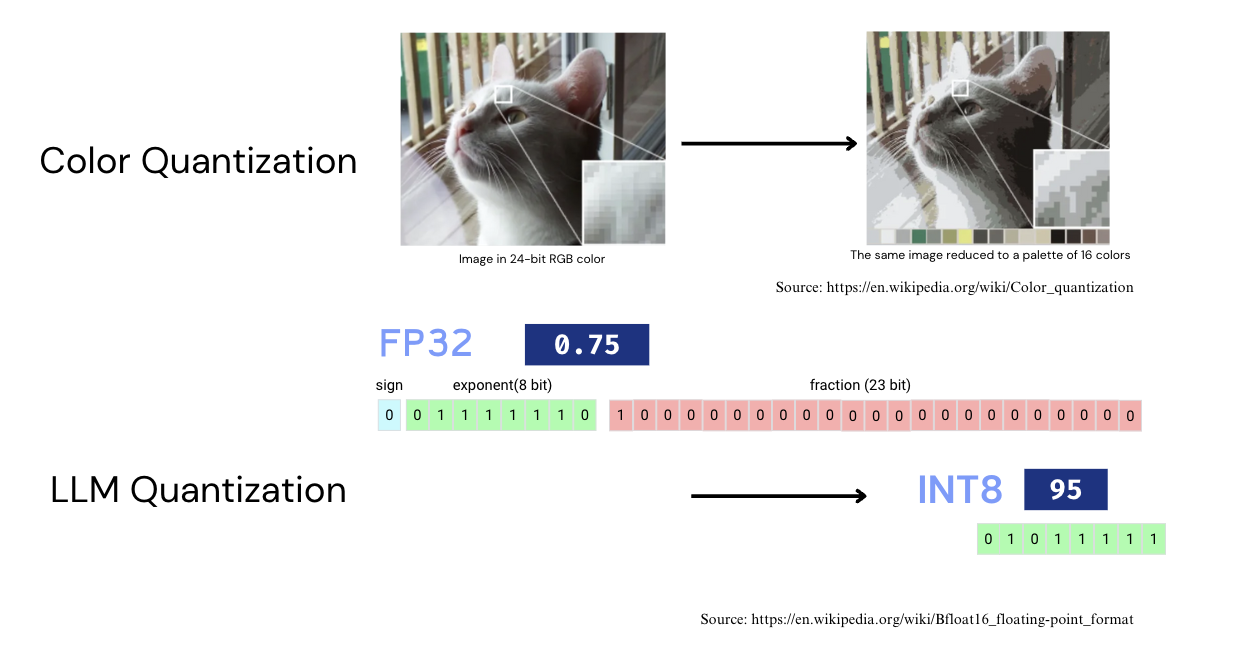
\includegraphics[width=\columnwidth]{img}
%     \caption{Analogy Between Color Quantization and LLM Quantization}
%     \label{fig:quantvisual}
% \end{figure}

Quantization can be applied 1) during the training phase (\textit{QAT}) which is observed to be highly efficient; however, due to significant resource demands, oftentimes appears impractical \cite{chen2024EfficientQAT}, and 2) post-training (\textit{PTQ}), which is more resource efficient, but can lead to certain levels of performance degradation \cite{shen2024exploring}. To break it down further, quantization granularity levels can vary from per-tensor (one step for the entire matrix), to per-token  (scales per output token) and per-channel (channel step size)\cite{shen2024exploring}. Based on the module of the model that is being quantized, we distinguish weight, activation and fixed-point quantization \cite{bai2024beyond}.

Having established the theoretical foundation of quantization, we now provide an overview of key methods. \textit{GPTQ} (Generative Pre-trained Transformers Quantization) focuses solely on weights and aims to minimize quantization error through optimal weight rounding \cite{frantar2023GPTQ}. In contrast, \textit{AWQ} (Activation-aware Weight Quantization) assumes that weights carry varying levels of importance, therefore skipping crucial activation outliers while aggressively quantizing the rest helps mitigate accuracy loss \cite{lin2024AWQ}. \textit{GGUF}, in turn a successor or deprecated \textit{GGML}, includes  quantization-aware kernels optimizations and  provides backward-compatible file format among other improvements \cite{rajput2024benchmarking}. SmoothQuant \cite{xiao2023SmoothQuant} enables quantization for both activations and weights by managing outlier values and QLoRA (4-bit quantized version of LoRA fine-tuning technique) \cite{dettmers2023qlora} reduces GPU requirements while still preserving performance.

Described techniques demonstrate superior advancements and efficiency, leading us to adopt GPTQ-, GGUF- and AWQ- quantized models in this study.

\section{Research Methodology}\label{method}

\subsection{Overview}

% Mariia
% • Describe and explain the research strategy (i.e. Surveys , Experiments , MSR , Case Study , Design Science , Action Research ). Motivate your choice of this method to address this problem.
% • Give a brief overview of the whole research method and the rest of the methodology section.
% • (For Experiments ) Describe independent/control/dependent variables, how the
% subjects were divided etc. Describe research questions as formal hypotheses

We perform \textbf{Experimentation}\cite{wohlin2012experimentation}, which is a research method, commonly used
to explore empirical correlations between several factors, in our case,
quantized LLMs and their ability to create REST links. By the nature of
experiment, we have control over subjects, objects and instrumentation in order
to manipulate experimental units and draw conclusions on dependent variable
output. Experiments are conducted to test the hypothesis and comparatively
access the impact of specific variables in a controlled setting, which is the
most suitable setup for answering our Research Questions.

Within a \textit{Controlled Experiment}, we aim to study the effect of \textit{Independent
Variables} (such as selected baseline LLM models and quantization techniques) on
\textit{Response Variables} (such as precision, recall, F1-score, and others)\cite{wohlin2012experimentation}. In the
design of the experiment we defined a number of treatments, specific
manipulations applied to subjects\cite{wohlin2012experimentation}.  In this case, \textit{treatments} involve a
comparative evaluation of LLama, Mistral, and Mixtral in both their
non-quantized and quantized versions for aligning Requirements and Test cases.
These models were established as a standard by Quinstedt et al. and Ivarsson et
al.\cite{quinstedt2024Optimizing},\cite{ivarsson2023automated} in their respective studies. 

% TODO: Ask Francisco about \textit{Hypothesis}
% Since we are focused on trade-offs, defining a binary hypothesis is tricky. *Do we need defined hypothesis for our research?*

% If yes, here are some possible ways to phrase it:
% -Increasing Variable A improves X but worsens Y.
% -There exists an optimal level of A that maximizes X while minimizing its negative impact on Y

% Added for A2 - Give a brief overview of the whole research method and the rest of the methodology section.
This section outlines the research type and structure, as well as evaluates the appropriateness of scope in connection to identified Research Questions. Data collection section defines procedures for sampling subjects of the study. Further we explain and motivate the choice of methods and statistical tests we use for data analysis and acknowledge identified threats to validity alongside mitigation strategies.

\begin{center}
   \begin{center}
        \textbf{Experiment Structure}
    \end{center}
    \begin{tcbraster}[raster columns=2, raster column skip=5pt, raster equal height=rows, raster row skip=5pt]
        \begin{roundedBox}
            \centering
            \textbf{Independent Variable (factors)}
            \begin{itemize}
                \item ``Base model''
                \item Level (treatment)
                    \begin{itemize}
                        \item GPTQ Quantization
                        \item GGUF Quantization
                        \item AWQ Quantization % Activation-aware Weight Quantization
                    \end{itemize}
            \end{itemize}
        \end{roundedBox}
        \begin{roundedBox}
            \centering
            \textbf{Objects (experimental units)}
            \begin{itemize}
                \item Hardware (Alvis)
                \item Alvis job-scripts
                \item REST-at tool
                % \item Hardware: local
            \end{itemize}
        \end{roundedBox}
        \begin{roundedBox}
            \centering
            \textbf{Dependent Variable (responses)}
            \begin{itemize}
                \item Accuracy
                \item Precision
                \item Recall
                \item $F1$-score
                \item Time-to-analyze
                \item GPU memory-usage (vRAM)
            \end{itemize}
        \end{roundedBox}
        \begin{roundedBox}
            \centering 
            \textbf{Control Variables (parameters)}
            \begin{itemize}
                \item Requirements file
                \item Test case file
                \item Ground truth file
                \item Prompt template
                \item Model hyper-parameters \\ (e.g. temperature)
                \item Python environment (version)
            \end{itemize}
        \end{roundedBox}
        \end{tcbraster}
        \begin{roundedBox}
            \centering
            \textbf{Output (artifacts)}
            \begin{itemize}
            \centering
                \item Structured trace links
                % (Req. --> Test cases)
            \end{itemize}
        \end{roundedBox}
\end{center}

\subsection{Data Collection}

% A) Describe and motivate data collection procedures, including how subjects are
% chosen (sampling), number of subjects, etc.
%   - Describe subjects (demographics, experience, etc.)
%
% B) Describe any instruments used in your study, e.g., interview guides,
% surveys, observation sheets, include these in your report (could be in appendix).
%
% C) Describe what types of data will be collected, is it qualitative,
% quantitative or both?
%
% D) What tooling, if any, will you use in the study (e.g., survey tool, MSR
% tool)
%
% E) Describe data collection procedures, sampling method(s), report the
% population and size of the sample.
% 
% F) If any instrument is used (e.g. document needed for the experiment,
% pre-questionnaire to check subjects background/experience, follow-up
% questionnaire), example questions/information from ALL of the needed instruments
% MUST be included.

% TODO: write about the datasets, where they come from and why its good.

Data (i.e. entries of requirement \& test pairs) are sampled from each dataset
to subsets ranging from 75 through 100 using the X method\footnote{LINK}.
There's not any subjects involved in this phase, apart from the authors of this
paper, who look over the experiments in the event of technical difficulties.

Furthermore, the prompts are outlined in the Appendix \ref{appendix}.
Environment details: ??

Overall, quantitative measures are gathered: (i) computed traces given (a) model
\& (b) dataset, (ii) benchmarks about job executions (e.g., running time,
consumed resources).

The revised \verb|REST-at| tool will primarily be used to gather the measures.
This will be done on the \verb|Alvis| platform.

Having obtained the measures, we utilize a \verb|Python| script that parses the
data to a more readable format. The script is too used for some additional 
analysis tasks\footnote{Point to a GitHub repo with the link}. % for analysis... (not during it)

Follow up on the environment. More about hardware + Avlis

\subsection{Data Analysis}
% Erik
% • Describe and motivate the methods for analysing the data
%  • Describe any quantitative data analysis that will be performed, if applicable.
%  – Describe the types of descriptive statistics you will use (e.g., data visualization, mean)
%  – This includes the types of statistical tests
%  and analysis you will apply and how you will interpret the results
% – Motivate the selection of statistical tests.

\textbf{TODO: add references! \cite{wohlin2012experimentation}}

non-parametric -- there are no assumptions on the distribution of the data / distribution is "even"

paired -- we are comparing pairs of data (rows)
% A   |   B
% ----------
% A1  |   B1
% A2  |   B2
% A3  |   B3

Are there 2 or more groups however? What happens when we use levels of treatment, i.e., different quantization methods? -- seems like we would have > 2 groups
% For the purposes of assignment 2 --> let's only use 2 groups
\begin{roundedBox}
\centering
    \textbf{groups $\textrangle$ 2 ? Friedman test : Wilcox rank sum test}  
\end{roundedBox}

The collected data will be analyzed using a \textbf{INSERT TEST METHOD}. The collected data is non-parametric---there are no \textbf{EGGSPLAIN WHY}---and paired---since we will be comparing the same tests (rows) between quantized and non-quantized model pairs.

Because of the stochastic nature of LLMs it is important that we perform repeated tests on the same input for each of the models in order to be able to include standard deviation measurements across the different metrics, this will allow us to reason about the consistency of each model as well as increase the validity of our measurements and subsequently our results.

\textbf{TODO: how will we represent the data?}
- tables good
- more?


\subsection{Threats to Validity}
% TOGETHER
% • Describe internal validity threats and mitigations.
% • Describe construct validity threats and mitigations.
% • Describe external validity threats and mitigations.
% • If applicable for your research method, describe further validity threats and mitigations under further categories.

% Ideas: 
Based on the guidelines proposed by Wohlin et al. \cite{wohlin2012experimentation} we identify the following threats to validity that might have influenced research findings: 
\subsection*{\textbf{1) Internal validity}}
    Response variability - due to stochastic behavior of LLMs, the same prompt can result in different outputs when executed several times, this behavior can not be mitigated. Instead, we try to eliminate it by invoking prompts multiple times and defining consistent hyper-parameters.
    
    Selection of models - proprietary/non-proprietary bias
    
    Quantization quality - if we use a pre-quantized model distributed via Hugging Face, there is a threat to quality/efficiency of quantization which directly impacts the results. alternative -> explore using Alvis for quantizing ourselves 

\subsection*{\textbf{2) External validity}}
    
    Domain-Specific Applicability - observed results might only be applicable within the explored domain due to the data specificity and scoped research questions.
    
    Results reproducibility on a local machine (depends on how we use Alvis)

\subsection*{\textbf{3) Construct validity}}
\textit{    *concerns generalisation of the experiment result to concept or theory behind the experiment*
}
Validity of test alignment provided by our Industry partner,  

\section*{Acknowledgment}
We dedicate our gratitude to our supervisor Francisco Gomes and responsible for the course in Research methods, Birgit Penzenstadler, for their valuable insights.

\subsection*{Assignment 1}

Breakdown of work:
\begin{itemize}
    \item Erik: \ref{background}, \ref{relatedWork} A
    \item Mariia: \ref{relatedWork} B and C
    \item Michal: \ref{intro} (+abstract)
\end{itemize}

Additionally, all members of the group collectively participated in literature
review, proof-reading, defining research-questions, and other tasks.

\bibliographystyle{IEEEtran}
\bibliography{lib}

\section*{Appendix}\label{appendix}

\end{document}